\documentclass[12pt, a4paper, addpoints]{exam}
% \documentclass[addpoints,answers]{exam}

\usepackage{mdframed} % Add this line in the preamble
% \usepackage{textcomp} % Required for \textcircled
% \usepackage{xfrac}
% \usepackage{xparse}
% \usepackage{xcolor}
\usepackage[utf8]{inputenc}
\usepackage[a4paper, margin=11mm]{geometry}
\usepackage{amsmath}

\usepackage[hidelinks]{hyperref}
\usepackage{enumitem}
\usepackage{multicol}
\usepackage{graphicx}
\usepackage{qrcode}
\usepackage{url}
\definecolor{GridColor}{gray}{.2}
\usepackage{tikz}
\usepackage{pgf}
\begin{document}

\newcommand{\labelslope}[6]{% Arguments: #1=grid width, #2=grid height, #3=xstart, #4=ystart, #5=xend, #6=yend
\begin{tikzpicture}
    % Draw a grid with size specified by #1 x #2
    \draw[step=1cm, gray, very thin] (0,0) grid (#1,#2);
    
    % Plot the line segment from (xstart, ystart) to (xend, yend)
    \draw[black, thick] (#3,#4) -- (#5,#6);
    
    % Calculate the horizontal (run) and vertical (rise) distances
    \pgfmathsetmacro{\run}{#5-#3}
    \pgfmathsetmacro{\rise}{#6-#4}
    
    % Draw the horizontal leg and label it
    \ifdim\run pt=0pt\else % Only draw if run is non-zero
        \draw[black, thick] (#3,#4) -- (#5,#4);
        \draw (#3,#4) -- (#5,#4) node[midway,below] {\large $\pgfmathprintnumber{\run}$};
    \fi
    
    % Draw the vertical leg and label it
    \ifdim\rise pt=0pt\else % Only draw if rise is non-zero
        \draw[black, thick] (#5,#4) -- (#5,#6);
        \draw (#5,#4) -- (#5,#6) node[midway,right] {\large $\pgfmathprintnumber{\rise}$};
    \fi
    
    % Add endpoints
    \filldraw [black] (#3,#4) circle (2pt); % Endpoint at starting point
    \filldraw [black] (#5,#6) circle (2pt); % Endpoint at ending point
\end{tikzpicture}
}

\newcommand{\gridslope}[6]{% Arguments: #1=grid size, #2=xstart, #3=ystart, #4=xend, #5=yend
\begin{tikzpicture}
    % Draw a grid with size specified by #1 x #2
    \draw[step=1cm, gray, very thin] (0,0) grid (#1,#2);
    
    % Plot the line segment from (xstart, ystart) to (xend, yend)
    \draw[black, thick] (#3,#4) -- (#5,#6);
    
    % Add endpoints
    \filldraw [black] (#3,#4) circle (2pt); % Endpoint at starting point
    \filldraw [black] (#5,#6) circle (2pt); % Endpoint at ending point
\end{tikzpicture}
}


\newcommand{\slopetool}[6]{% Arguments: #1=grid size x, #2=grid size y, #3=xstart, #4=ystart, #5=xend, #6=yend
\begin{tikzpicture}
    % Draw a grid with size specified by #1 x #2
    \draw[step=1cm, gray, very thin] (0,0) grid (#1,#2);

    % Draw x and y axes
    \draw[->, thick] (0,0) -- (#1+0.5,0) node[anchor=north] {x};
    \draw[->, thick] (0,0) -- (0,#2+0.5) node[anchor=east] {y};

    % Add scale markers on x and y axes
    \foreach \x in {1,2,...,#1} \draw (\x,0) -- (\x,-0.1) node[anchor=north] {\x};
    \foreach \y in {1,2,...,#2} \draw (0,\y) -- (-0.1,\y) node[anchor=east] {\y};

    % Plot the line segment from (xstart, ystart) to (xend, yend)
    \draw[black, thick] (#3,#4) -- (#5,#6);

    % Draw the right triangle formed by the line segment and axes
    \draw[black, thick] (#3,#4) -- (#5,#4);
    \draw[black, thick] (#5,#4) -- (#5,#6);

    % Add endpoints
    \filldraw [black] (#3,#4) circle (2pt); % Endpoint at starting point
    \filldraw [black] (#5,#6) circle (2pt); % Endpoint at ending point
\end{tikzpicture}
}

\input{linesegment}

\pgfmathsetseed{\number\pdfrandomseed}
% \pointsonrightmargin
% \nopointsinmargin 

% Redefine the point display command to show nothing next to the question
% \renewcommand{\pointformat}{}

\begin{minipage}[t]{0.2\textwidth} 
  % \includegraphics[width=1\lineswidth]{images/logo.jpg}\hspace{17mm}
   \qrcode[height=30mm]{https://www.geogebra.org/m/bdcutx2w#chapter/1044119} 
\end{minipage}
\begin{minipage}[t]{.5\textwidth} 
\vspace{-16mm}
{\huge 
   {\LARGE\textbf{Positive Slopes on a Grid
}\\
   Learn by Doing \\
QR for Slope Chapter \\
   \today}
   }  
\end{minipage}
\begin{minipage}[t]{0.3\textwidth} 
   % \includegraphics[width=\linewidth]{images/logo.jpg}
\end{minipage}
\begin{mdframed}[backgroundcolor=gray!20] % Light grey background
 \textbf{Slope} is the \textit{steepness} of a line segment. It measures how much a line rises vertically between two points in a horizontal run. We learn to use a \textbf{slope triangle}  to calculate slope values.

There are four types of slope:Positive,  Negative, Zero and Undefined Slope.


In this lesson, we look at \textbf{Positive Slopes}.  Line segments that rise from left to right and are also called  \textit{increasing line segments}. 

To express slope mathematically, we use the formula:
\[ \text{slope} (m) = \frac{\text{rise}}{\text{run}} \]

Here, the slope is denoted by the variable letter \(m\).
\end{mdframed}






\begin{questions}



\newcommand{\smallspace}{\vspace{1mm}}


\question Find the slope using the rise and run?
\begin{multicols}{3}
\begin{parts}

\part \scalebox{0.8}{\labelslope
{5}{5}
{0}{1}
{5}{5}} 
\part \scalebox{0.8}{\labelslope
{5}{5}
{0}{5}
{4}{0}} 
\part \scalebox{0.8}{\labelslope
{5}{5}
{1}{4}
{4}{0}} 
% \part \scalebox{0.8}{\labelslope
% {5}{5}
% {2}{1}
% {5}{5}}
% \part \scalebox{0.8}{\labelslope{5}{5}{0}{0}{3}{1}} 

\end{parts}
\end{multicols}




\renewcommand{\smallspace}{\vspace{4mm}}
\question Find the slope using the rise and run?
\begin{multicols}{3}
\begin{parts}
\part \slopetool{5}{5}{0}{0}{2}{5} \smallspace
\part \slopetool{5}{5}{0}{3}{5}{5}\smallspace
\part \slopetool{5}{5}{0}{0}{5}{1} \smallspace

\end{parts}
\end{multicols}


\renewcommand{\smallspace}{\vspace{4mm}}






\newcommand{\gridblank}[5]{% Arguments: #1=grid width, #2=grid height, #3=sign of slope (either {} for positive or {-} for negative), #4=numerator, #5=denominator
\begin{tikzpicture}
    % Draw a grid with size specified by #1 x #2
    \draw[step=1cm, gray, very thin] (0,0) grid (#1,#2);
    
    % Write the slope below the grid, including the sign directly from #3
    \node at (#1/2, -0.75) {Slope: $#3\dfrac{#4}{#5}$};
\end{tikzpicture}
}



\begin{mdframed}[backgroundcolor=gray!20] % Light grey background
Up to now  we converted slope from a number to a graph and now we will do this backwards.
\end{mdframed}



For a slope of \(m = \frac{3}{4}\), start at \(A(0, 0)\) so you can go to the right and up.


As a picture it looks like:  


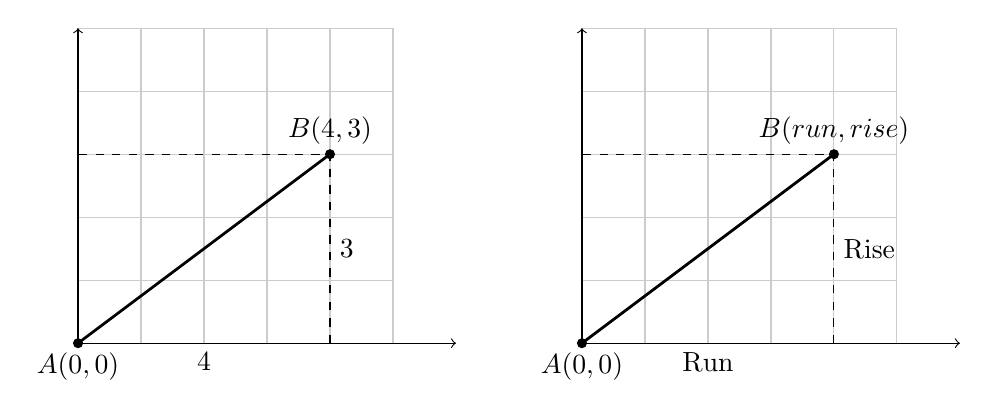
\begin{tikzpicture}[scale=0.8]
    % Original graph with slope triangle labeled 3 and 4 and coordinates at (0,0)
    \begin{scope}[shift={(0,0)}]
        \draw[thin,gray!40] (0,0) grid (5,5);
        \draw[<->] (0,5) -- (0,0) -- (6,0);
        \filldraw[black] (0,0) circle(2pt) node[anchor=north] {$A(0,0)$};
        \filldraw[black] (4,3) circle(2pt) node[anchor=south] {$B(4,3)$};
        \draw[line width=1pt] (0,0) -- (4,3);
        \draw[dashed] (4,0) -- (4,3) -- (0,3);
        \draw (4,1.5) node[right] {$3$}; % Rise
        \draw (2,0) node[below] {$4$}; % Run
    \end{scope}
    
    % Modified graph with "run,rise" labeled and coordinates at (0,0)
    \begin{scope}[shift={(8,0)}]
        \draw[thin,gray!40] (0,0) grid (5,5);
        \draw[<->] (0,5) -- (0,0) -- (6,0);
        \filldraw[black] (0,0) circle(2pt) node[anchor=north] {$A(0,0)$};
        \filldraw[black] (4,3) circle(2pt) node[anchor=south] {$B(run,rise)$};
        \draw[line width=1pt] (0,0) -- (4,3);
        \draw[dashed] (4,0) -- (4,3) -- (0,3);
        \draw (4,1.5) node[right] {Rise}; % Rise
        \draw (2,0) node[below] {Run}; % Run
    \end{scope}
\end{tikzpicture}
\question 
Construct a line segment to represent a positive slope \(m\).








\begin{multicols}{3}
\begin{parts}
\part \gridblank{5}{5}{}{1}{5}
\part \gridblank{5}{5}{}{2}{5}
\part \gridblank{5}{5}{}{3}{5}
\part \gridblank{5}{5}{}{4}{5}
\part \gridblank{5}{5}{}{1}{4} 
\part \gridblank{5}{5}{}{3}{4} 
\part \gridblank{5}{5}{}{5}{4}
\part \gridblank{5}{5}{}{2}{3}
% \part \gridblank{5}{5}{}{1}{3} 
% \part \gridblank{5}{5}{}{4}{3} 
% \part \gridblank{5}{5}{}{5}{3}
% \part \gridblank{5}{5}{}{1}{2}
% \part \gridblank{5}{5}{}{3}{2}
% \part \gridblank{5}{5}{}{5}{2}
% \part \gridblank{5}{5}{}{0}{2}
% \part \gridblank{5}{5}{-}{5}{4}
% \part \gridblank{5}{5}{}{4}{2}
\part \gridblank{5}{5}{-}{1}{2}
\end{parts}
\end{multicols}





\end{document}
